% \section{Atividades}
%
% Neste módulo, foram realizadas atividades práticas voltadas à análise de regras
% de firewall, filtragem de tráfego de rede, manipulação de resolução DNS,
% estabelecimento de túneis VPN e controle de pacotes ICMP em ambientes
% \textit{Kali Linux} e \textit{Windows Server 2022}.
%
% As atividades envolveram a exploração das listas de controle de acesso (ACL)
% no firewall avançado do Windows Server 2022, a aplicação de regras com
% \textit{iptables} para bloqueio de sites, redirecionamento de consultas DNS,
% uso de conexão segura via \textit{OpenVPN} e bloqueio seletivo de mensagens
% ICMP em rede local.
%
% Cada atividade apresenta abaixo o respectivo print solicitado, acompanhado de
% descrição explicativa conforme exigido nas orientações do módulo.
%
% \newpage
%
\question[Atividade 11.6]{Explorando ACL no Firewall do Windows Server 2022}

\begin{figure}[H]
\centering
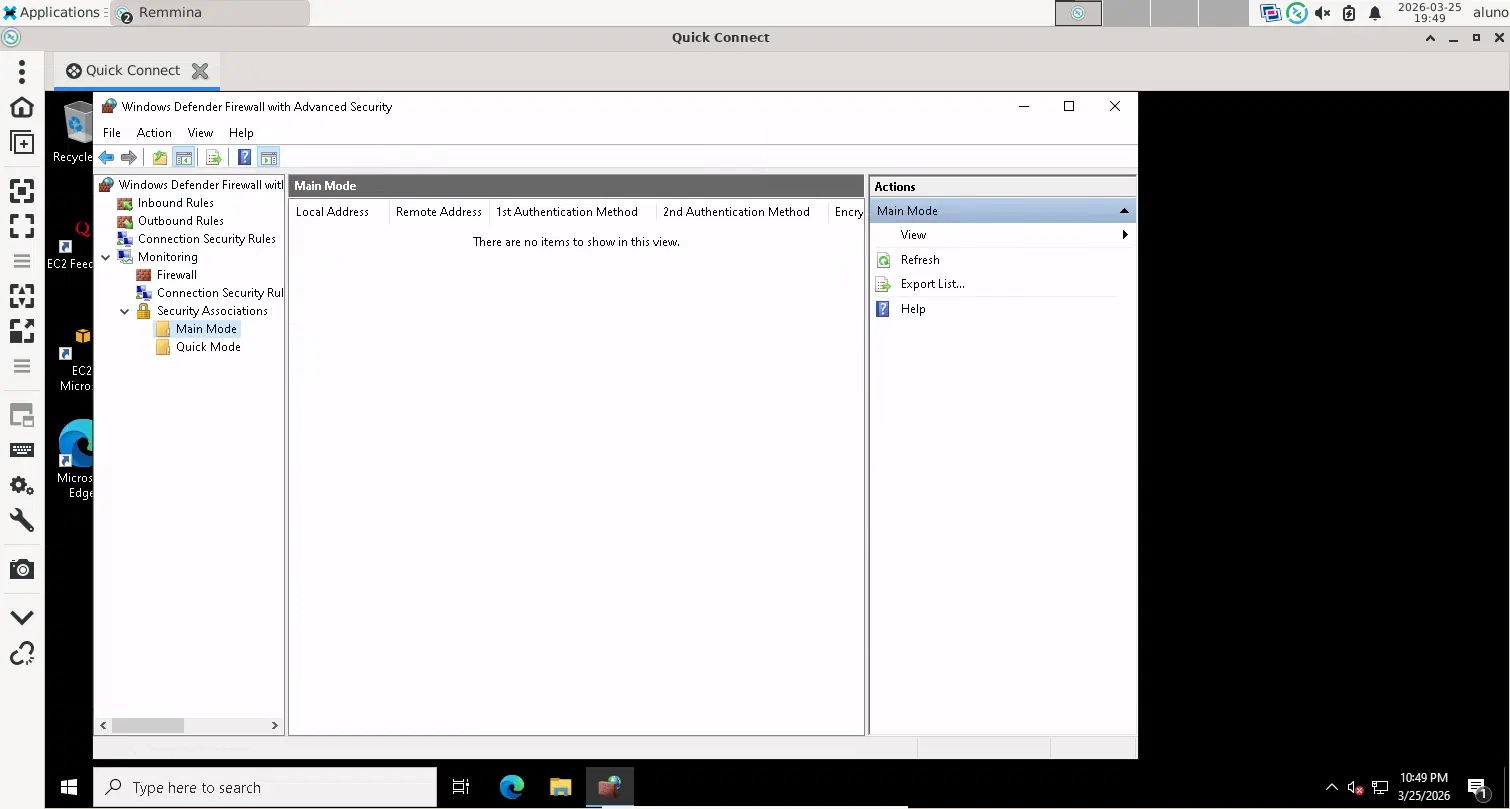
\includegraphics[width=0.99\textwidth]{./fig/fig11.6.png}
\caption{Visualização da seção Main Mode em Security Associations no firewall avançado do Windows Server 2022}
\label{fig:fig11.6}
\end{figure}

\newpage

\question[Atividade 11.7]{Bloqueando sites usando iptables no Kali Linux}

\begin{figure}[H]
\centering
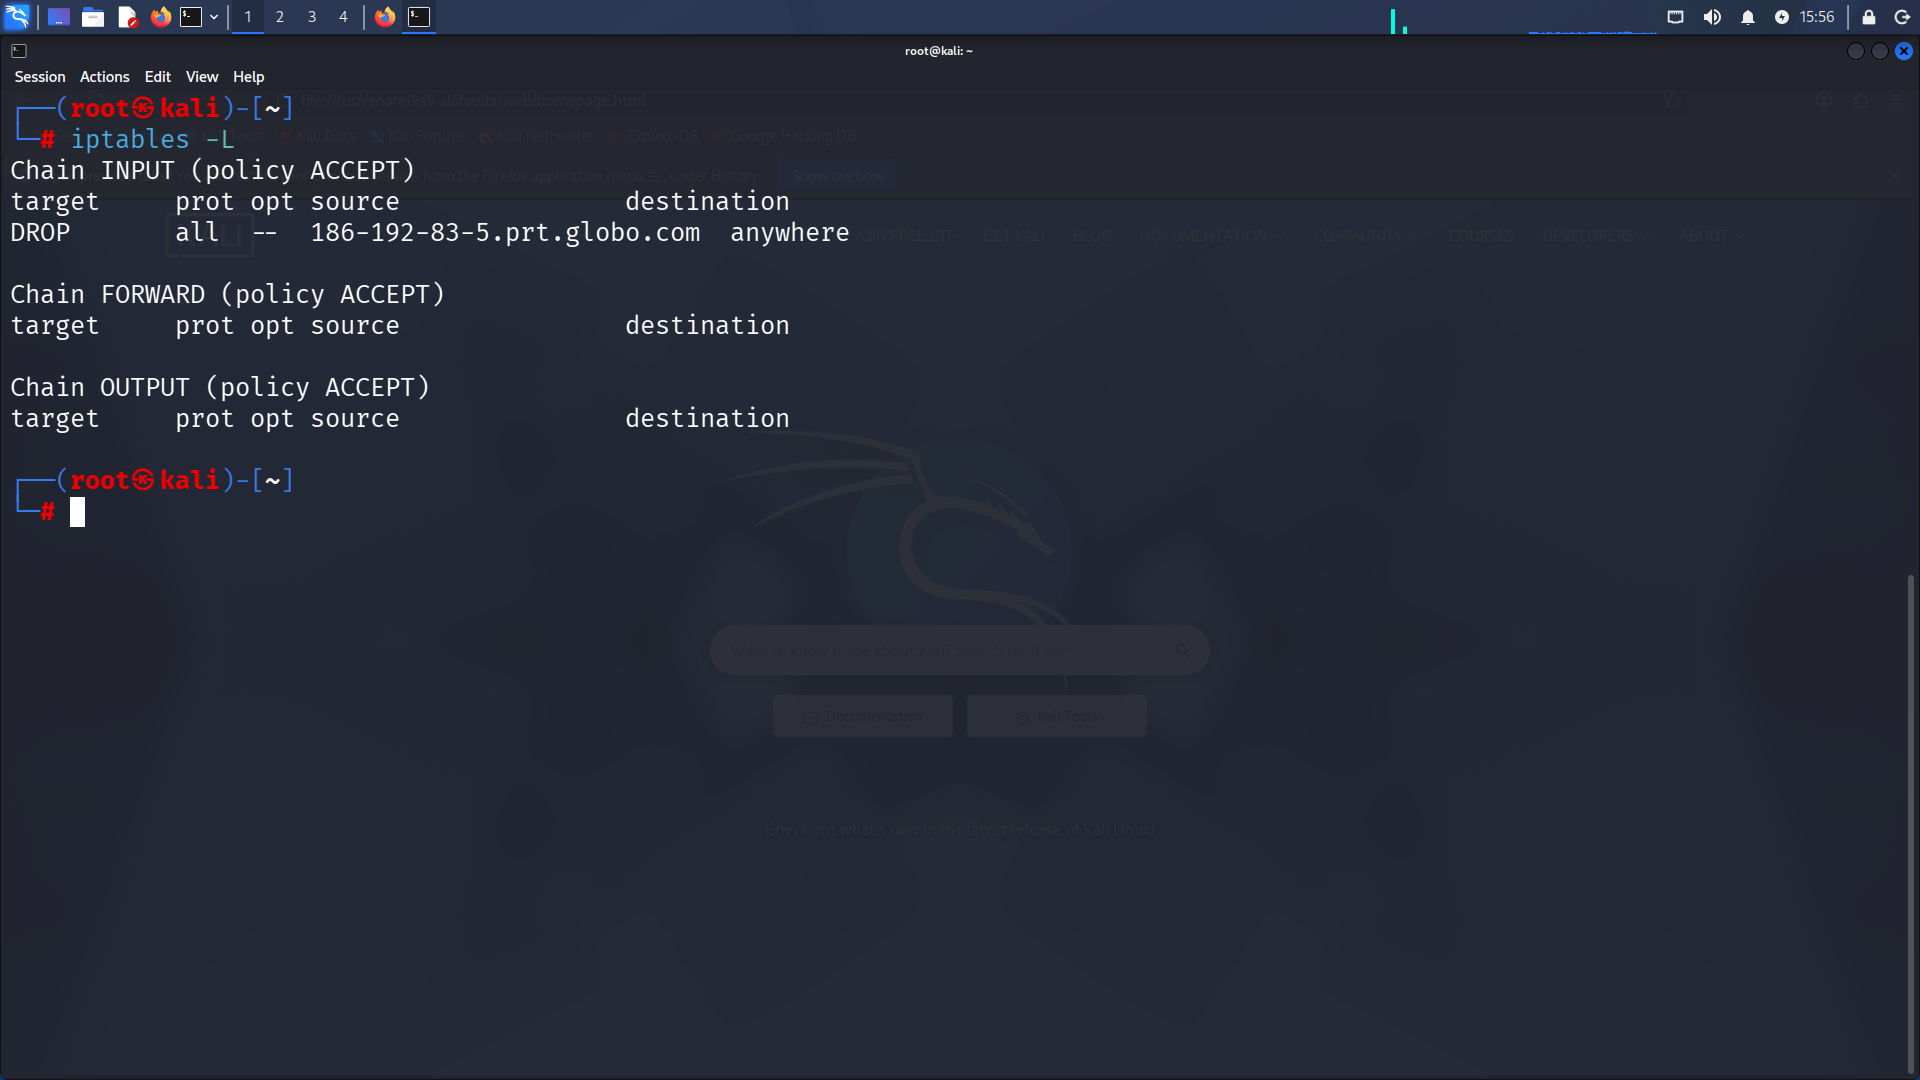
\includegraphics[width=0.99\textwidth]{./fig/fig11.7.png}
\caption{Listagem das regras do iptables contendo bloqueio aplicado ao domínio globo.com.br}
\label{fig:fig11.7}
\end{figure}

\newpage

\question[Atividade 11.8]{Redirecionando requisições DNS usando iptables no Kali Linux}

\begin{figure}[H]
\centering
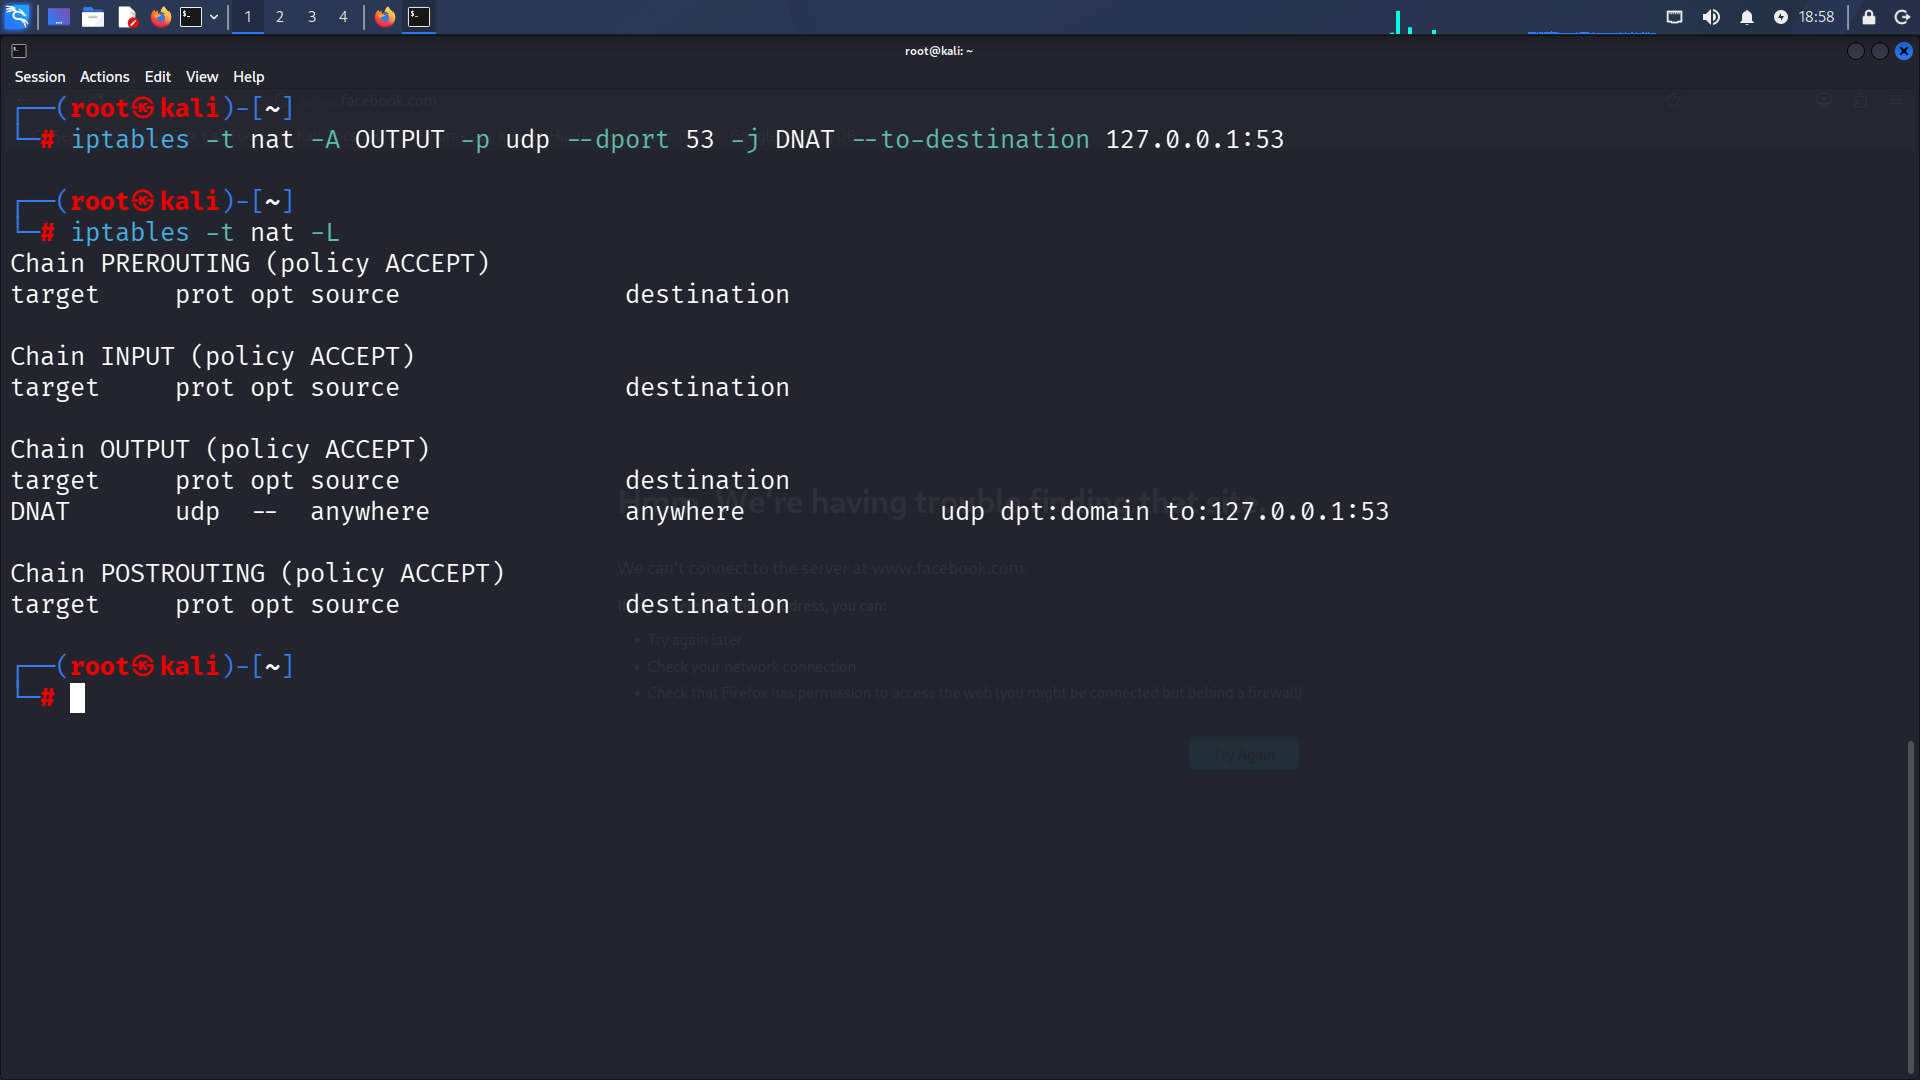
\includegraphics[width=0.99\textwidth]{./fig/fig11.8.png}
\caption{Regra NAT do iptables redirecionando tráfego DNS para 127.0.0.1}
\label{fig:fig11.8}
\end{figure}

\newpage

\question[Atividade 11.9]{Usando OpenVPN no Kali Linux}

\begin{figure}[H]
\centering
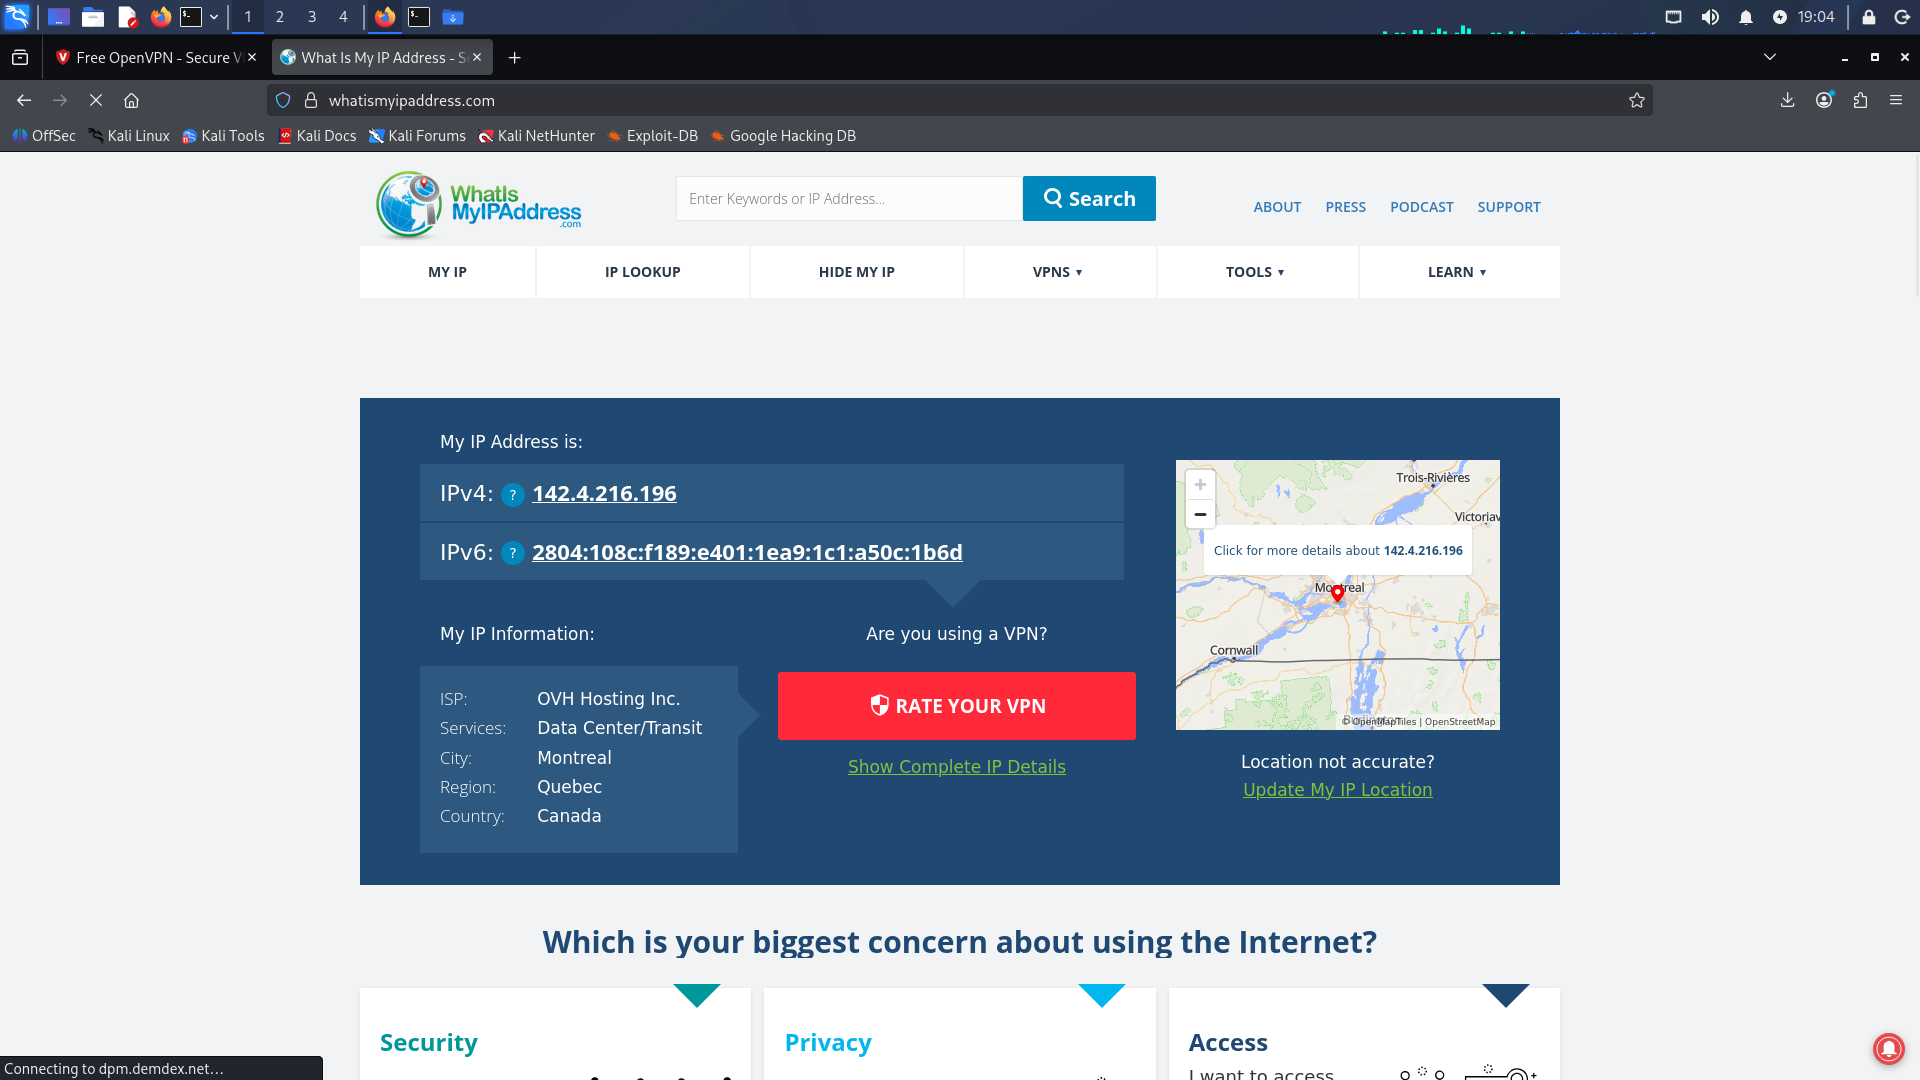
\includegraphics[width=0.99\textwidth]{./fig/fig11.9.png}
\caption{Verificação do IP público após conexão OpenVPN com saída internacional}
\label{fig:fig11.9}
\end{figure}

\newpage

\question[Atividade 11.10]{Bloqueando pacotes ICMP provenientes do Windows Server 2022}

\begin{figure}[H]
\centering
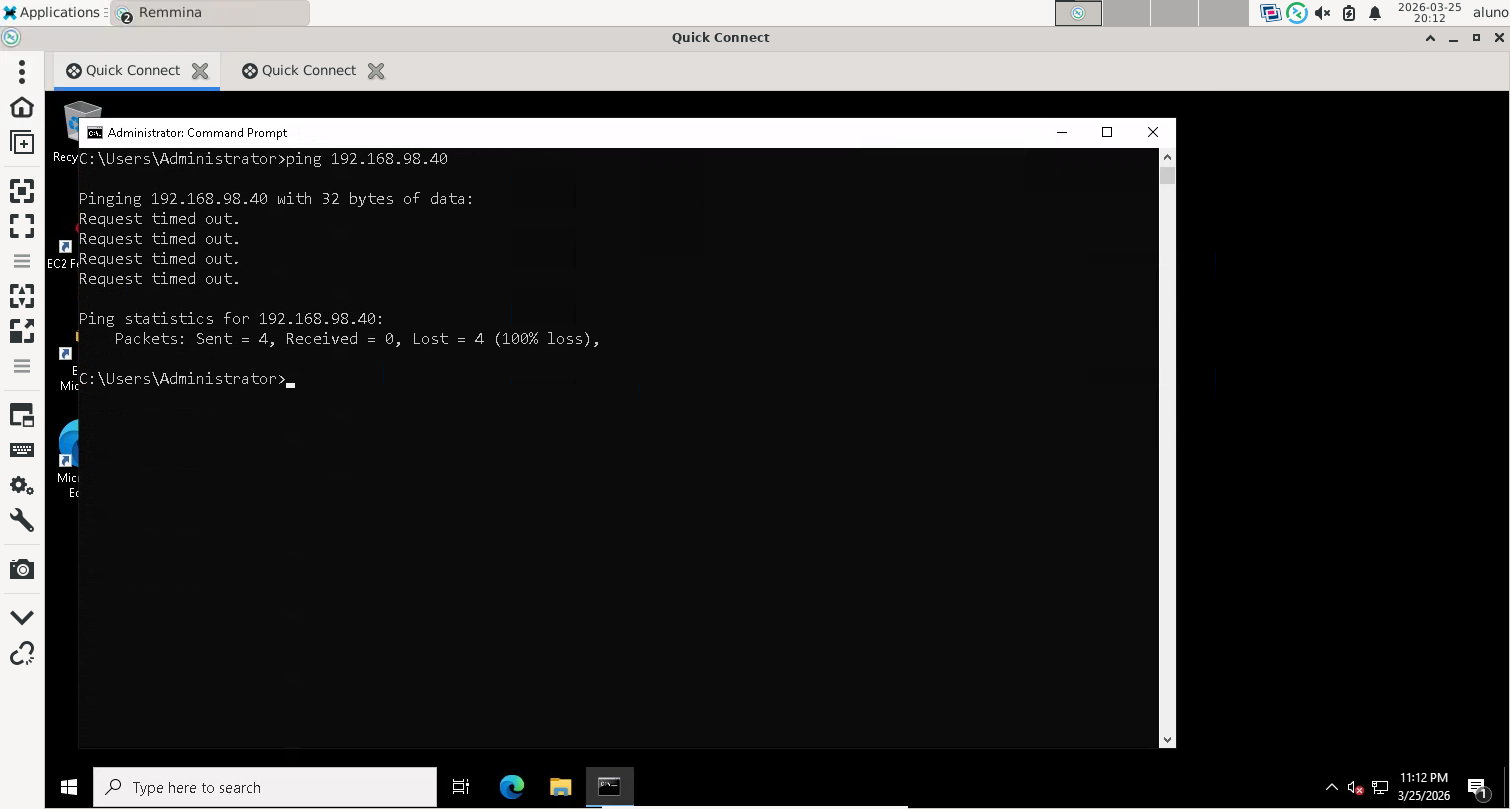
\includegraphics[width=0.99\textwidth]{./fig/fig11.10.png}
\caption{Falha de resposta ICMP após bloqueio aplicado com iptables no Kali Linux}
\label{fig:fig11.10}
\end{figure}
